\documentclass[a4paper]{article}
\usepackage[utf8]{inputenc}
\usepackage{amsmath}
\usepackage{amssymb}
\usepackage{caption}
\usepackage{mathtools}
\usepackage{amsfonts}
\usepackage{lastpage}
\usepackage{tikz}
\usepackage{float}
\usepackage{textcomp}
\usetikzlibrary{patterns}
\usepackage{pdfpages}
\usepackage{gauss}
\usepackage{fancyvrb}
\usepackage[table]{colortbl}
\usepackage{fancyhdr}
\usepackage{graphicx}
\usepackage[margin=2.5 cm]{geometry}

\definecolor{listinggray}{gray}{0.9}
\usepackage{listings}
\lstset{
	language=,
	literate=
		{æ}{{\ae}}1
		{ø}{{\o}}1
		{å}{{\aa}}1
		{Æ}{{\AE}}1
		{Ø}{{\O}}1
		{Å}{{\AA}}1,
	backgroundcolor=\color{listinggray},
	tabsize=3,
	rulecolor=,
	basicstyle=\scriptsize,
	upquote=true,
	aboveskip={0.2\baselineskip},
	columns=fixed,
	showstringspaces=false,
	extendedchars=true,
	breaklines=true,
	prebreak =\raisebox{0ex}[0ex][0ex]{\ensuremath{\hookleftarrow}},
	frame=single,
	showtabs=false,
	showspaces=false,
	showlines=true,
	showstringspaces=false,
	identifierstyle=\ttfamily,
	keywordstyle=\color[rgb]{0,0,1},
	commentstyle=\color[rgb]{0.133,0.545,0.133},
	stringstyle=\color[rgb]{0.627,0.126,0.941},
  moredelim=**[is][\color{blue}]{@}{@},
}

\lstdefinestyle{base}{
  emptylines=1,
  breaklines=true,
  basicstyle=\ttfamily\color{black},
}

\pagestyle{fancy}
\def\checkmark{\tikz\fill[scale=0.4](0,.35) -- (.25,0) -- (1,.7) -- (.25,.15) -- cycle;}
\newcommand*\circled[1]{\tikz[baseline=(char.base)]{
            \node[shape=circle,draw,inner sep=2pt] (char) {#1};}}
\newcommand*\squared[1]{%
  \tikz[baseline=(R.base)]\node[draw,rectangle,inner sep=0.5pt](R) {#1};\!}
\newcommand{\comment}[1]{%
  \text{\phantom{(#1)}} \tag{#1}}
\def\el{[\![}
\def\er{]\!]}
\def\dpip{|\!|}
\def\MeanN{\frac{1}{N}\sum^N_{n=1}}
\cfoot{Page \thepage\ of \pageref{LastPage}}
\DeclareGraphicsExtensions{.pdf,.png,.jpg}
\author{Nikolaj Dybdahl Rathcke (rfq695)}
\title{Signal and Image Processing \\ Assignment 3}
\lhead{SIP}
\rhead{Assignment 3}

\begin{document}
\maketitle

\section{Fourier transform - Theory}
\subsection{(a)}
Fourier series is a way to represent periodic functions by a, potentially infinite, sum of complex exponentials (namely sine and cosine functions) of discrete frequencies. The fourier transform is the extension of this to non-periodic function as well, but it transforms the signal from the time domain into a frequency domain, by breaking it into the frequencies that exists in the signal.

\subsection{(b)}
The fourier transform of $f(x)$ is given by:
\begin{align*}
  F(k_x)=\frac{1}{2\pi}\int_{-\infty}^{\infty}f(x)e^{-ik_xx}dx
\end{align*}
We want to show that the transformation of $f(x)$ when it is real and even is also real and even. Euler's formula states that for any real $x$:
\begin{align*}
  e^{ix}=\cos(x)+i\sin(x)
\end{align*}
Since the function is real, this means $i=0$ and we can say:
\begin{align*}
  F(k_x)=\frac{1}{2\pi}\int_{-\infty}^{\infty}f(x)\cos(k_xx)dx
\end{align*}
This means the integral over $f(x)cos(k_xx)$ must be real as it is the product of two real functions. Now, we prove that if $f(x)$ is even, then so is the transformation. If a function is even, the following holds:
\begin{align*}
  g(x)=g(-x)
\end{align*}
We want to prove this for when the fourier transform is the function $g$. We let $u=-x$ and $dx=-du$. We can then write:
\begin{align*}
  F(-k_x)&= \frac{1}{2\pi}\int_{-\infty}^{\infty}f(-u)e^{-i(-k_x)x}du \\
         &= \frac{1}{2\pi}\int_{-\infty}^{\infty}f(-u)e^{ik_xx}du \\
  &= F(k_x)
\end{align*}
these two derivation prove that the fourier transformation of a real and even function is also real and even.

\subsection{(c)}
Again we use the fourer transform of $f(x)$ where $f(x)=\delta(x-d)+\delta(x+d)$, so
\begin{align*}
  F(k_x)=\frac{1}{2\pi}\int_{-\infty}^{\infty}(\delta(x-d)+\delta(x+d))e^{-ik_xx}dx
\end{align*}
We can split this into two integrals:
\begin{align*}
  F(k_x)=\frac{1}{2\pi}\left(\int_{-\infty}^{\infty}\delta(x-d)e^{-ik_xx}dx+\int_{-\infty}^{\infty}\delta(x+d)e^{-ik_xx}dx\right)
\end{align*}
Now the shifting property, which states that $\int_{-\infty}^{\infty}f(x)\delta(x-d)dx=f(d)$, allows us to write:
\begin{align*}
  F(k_x)=\frac{1}{2\pi}\left(e^{-ik_xd}+e^{-ik_x(-d)}\right)
\end{align*}
We can simplify this further by rewriting the complex exponentials using Euler's formula:
\begin{align*}
  F(k_x)&= \frac{1}{2\pi}\left(\cos(k_xd)-i\sin(k_xd)+\cos(-k_xd)-i\sin(-k_xd)\right) \\
        &= \frac{1}{2\pi}\left(2\cos(k_xd)-i(\sin(-k_xd)+\sin(k_xd))\right) \comment{As cosine is even} \\
        &= \frac{1}{2\pi}\left(2\cos(k_xd)\right) \comment{As sine is odd} \\
        &= \frac{\cos(k_xd)}{\pi}
\end{align*}
which is the derivation of the continuous fourier transform of $\delta(x-d)+\delta(x+d)$ for some $d$.

\subsection{(d)}
\subsubsection{(i)}
We can easily show the integral is $1$. The function is a constant function taking value $1/a$ for $x=-a/2$ to $a/2$. This is, as the name implies, a box of with length $2\cdot 2/a$ (both sides of the $y-axis$ and height $1/a$. This yields an area (which is what the integral is) of
\begin{align*}
  2\cdot \frac{a}{2} \cdot \frac{1}{a} = \frac{2a}{2a} = 1
\end{align*}
And we have shown the integral of the box function is $1$.

\subsubsection{(ii)}
We have that the fourier transform is given by:
\begin{align*}
  F(k_x)=\frac{1}{2\pi}\int_{-\infty}^{\infty}f(x)e^{-ik_xx}dx
\end{align*}
Since the function only takes values other than $0$ in the interval $[-a/2, a/2]$, we can write $B(k)$ as:
\begin{align*}
  B(k)=\frac{1}{2\pi}\int_{-a/2}^{a/2}f(x)e^{-ikx}dx
\end{align*}
We can now insert the the box function:
\begin{align*}
  B(k)&=\frac{1}{2\pi}\int_{-a/2}^{a/2}\frac{1}{a}e^{-ikx}dx \\
        &= \frac{1}{2\pi a} \int_{-a/2}^{a/2}e^{-ikx}dx \\
        &= \frac{1}{2\pi a} \int_{-a/2}^{a/2}\cos(kx)-i\sin(kx)dx \\
        &= \frac{1}{2\pi a}\frac{2\sin(\frac{ak}{2})}{k} \comment{As the definite integral is $\frac{2\sin(\frac{ak}{2})}{k}$} \\
        &= \frac{1}{\pi ak}\sin\left(\frac{ak}{2}\right)
\end{align*}
Which is what we wanted to show. To rewrite $B(k)$ using \texttt{sinc}, we want to produce $\frac{ak}{2}$ in the denominator. So,
\begin{align*}
  B(k)&= \frac{1}{\pi ak}\sin\left(\frac{ak}{2}\right) \\
      &= \frac{1}{\pi}\frac{\sin(\frac{ak}{2})}{ak} \\
      &= \frac{1}{\pi}\frac{\sin(\frac{ak}{2})}{\frac{ak}{2}}\frac{1}{2} \comment{Extending fraction with $1/2$} \\
      &= \frac{1}{2\pi}\text{sinc}\left(\frac{ak}{2}\right) \comment{Using \texttt{sinc}}
\end{align*}
Which is $B(k)$ expressed with a \texttt{sinc} term.

\subsubsection{(iii)}
We want to show that $B(k)$ approached $\frac{1}{2\pi}$ when $a$ approaches infinity. By definition, the sinc term approaches $1$ when $\frac{ak}{2}$ approaches zero. As we let $a\rightarrow 0$, it is indeed true that the fraction approaches $0$, thusi we can replace the sinc term by $1$:
\begin{align*}
  \lim_{a\rightarrow 0}B(k)&=\frac{1}{2\pi}\text{sinc}\left(\frac{ak}{2}\right) \\
                           &= \frac{1}{2\pi}
\end{align*}
Which is what we wanted to show. This proves the first entry in Table 5.2. As we let $a$ approach $0$, the box's length will also approach $0$, which correspond to the delta dirac function since the integral over the function remains $1$.

\subsubsection{(iv)}
A function and it's fourier transform cannot both have compact support as implied by the Paley-Wiener theorem. This is because the fourier transform of a function with compact support is an entire function, which in return means that the fourier transform can not have compact support.

\section{Fourier Transform - Practice}
\subsection{(a)}
The code for this question is seen below:
\lstinputlisting[language=Matlab]{src/q2_1.m}
The function \texttt{fft} is the fast fourier transformation in Matlab, which splits the signal into frequencies. The function \texttt{fftshift} shifts by moving the zero-frequency component to the center, which is useful four visualizing a fourier transform. Since the resulting power spectrum is pretty obscure, the logarithm is taken of the spectrum, which gives a more interpretable spectrum as the difference between high and low frequencies is clearer. Figure \ref{fig1} shows the original image along with its resulting power spectrum.
\begin{figure}[H]
  \centering
  \captionsetup{justification=centering}
  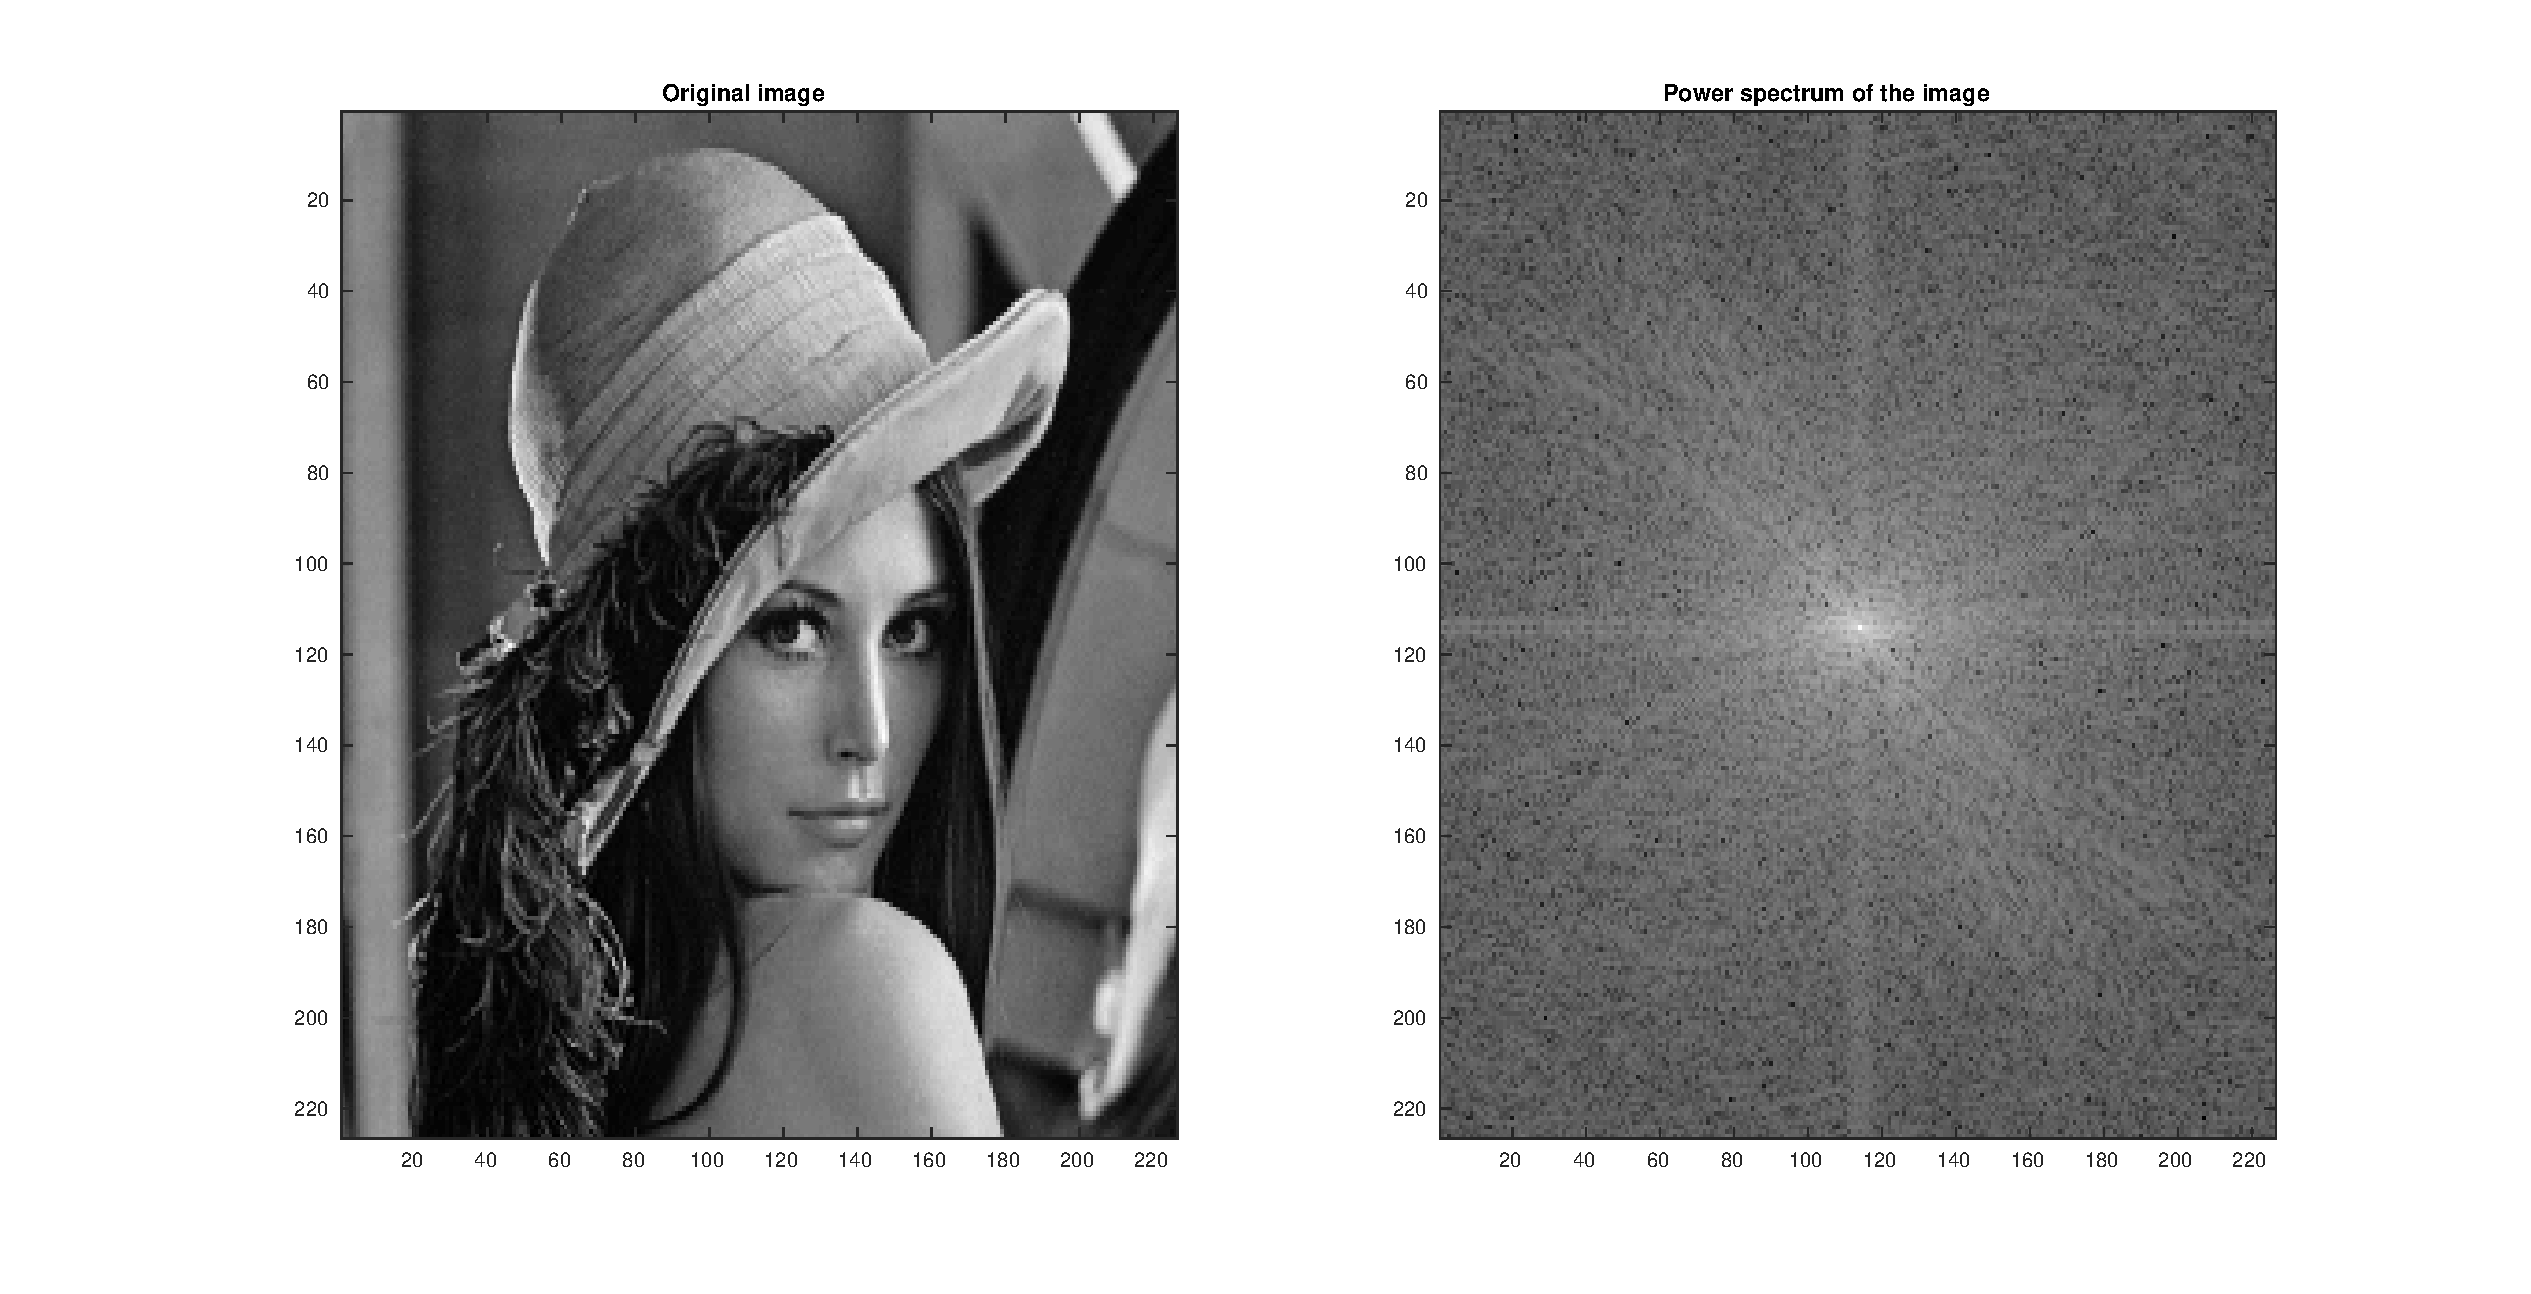
\includegraphics[width=\textwidth]{fig1.eps}
  \caption{Figure showing the original image \texttt{lena.tiff} and the power spectrum generated from the picture.}
  \label{fig1}
\end{figure}
The power spectrum is useful for determining what frequencies are dominant. A pixel's distance to the center is an indication of its frequency. \\
The "plus" of bright light we can see go through the center is because we shift the image, which means it is the edges we can see in the middle. The diagonal line we can see could come from the bottom of the hat. Another thing to note, is that it is very bright in the center, which means the low frequencies are very dominant in the image.

\subsection{(b)}
The code for this question be seen below:
\lstinputlisting[language=Matlab]{src/q2_2.m}
The function \texttt{nestedConv} performs convolution with nested for loops while the function \texttt{fourConv} performs convolution with FFT. By running function \texttt{q2\_2a}, we get the result in Figure \ref{fig2_2a}.
\begin{figure}[H]
  \centering
  \captionsetup{justification=centering}
  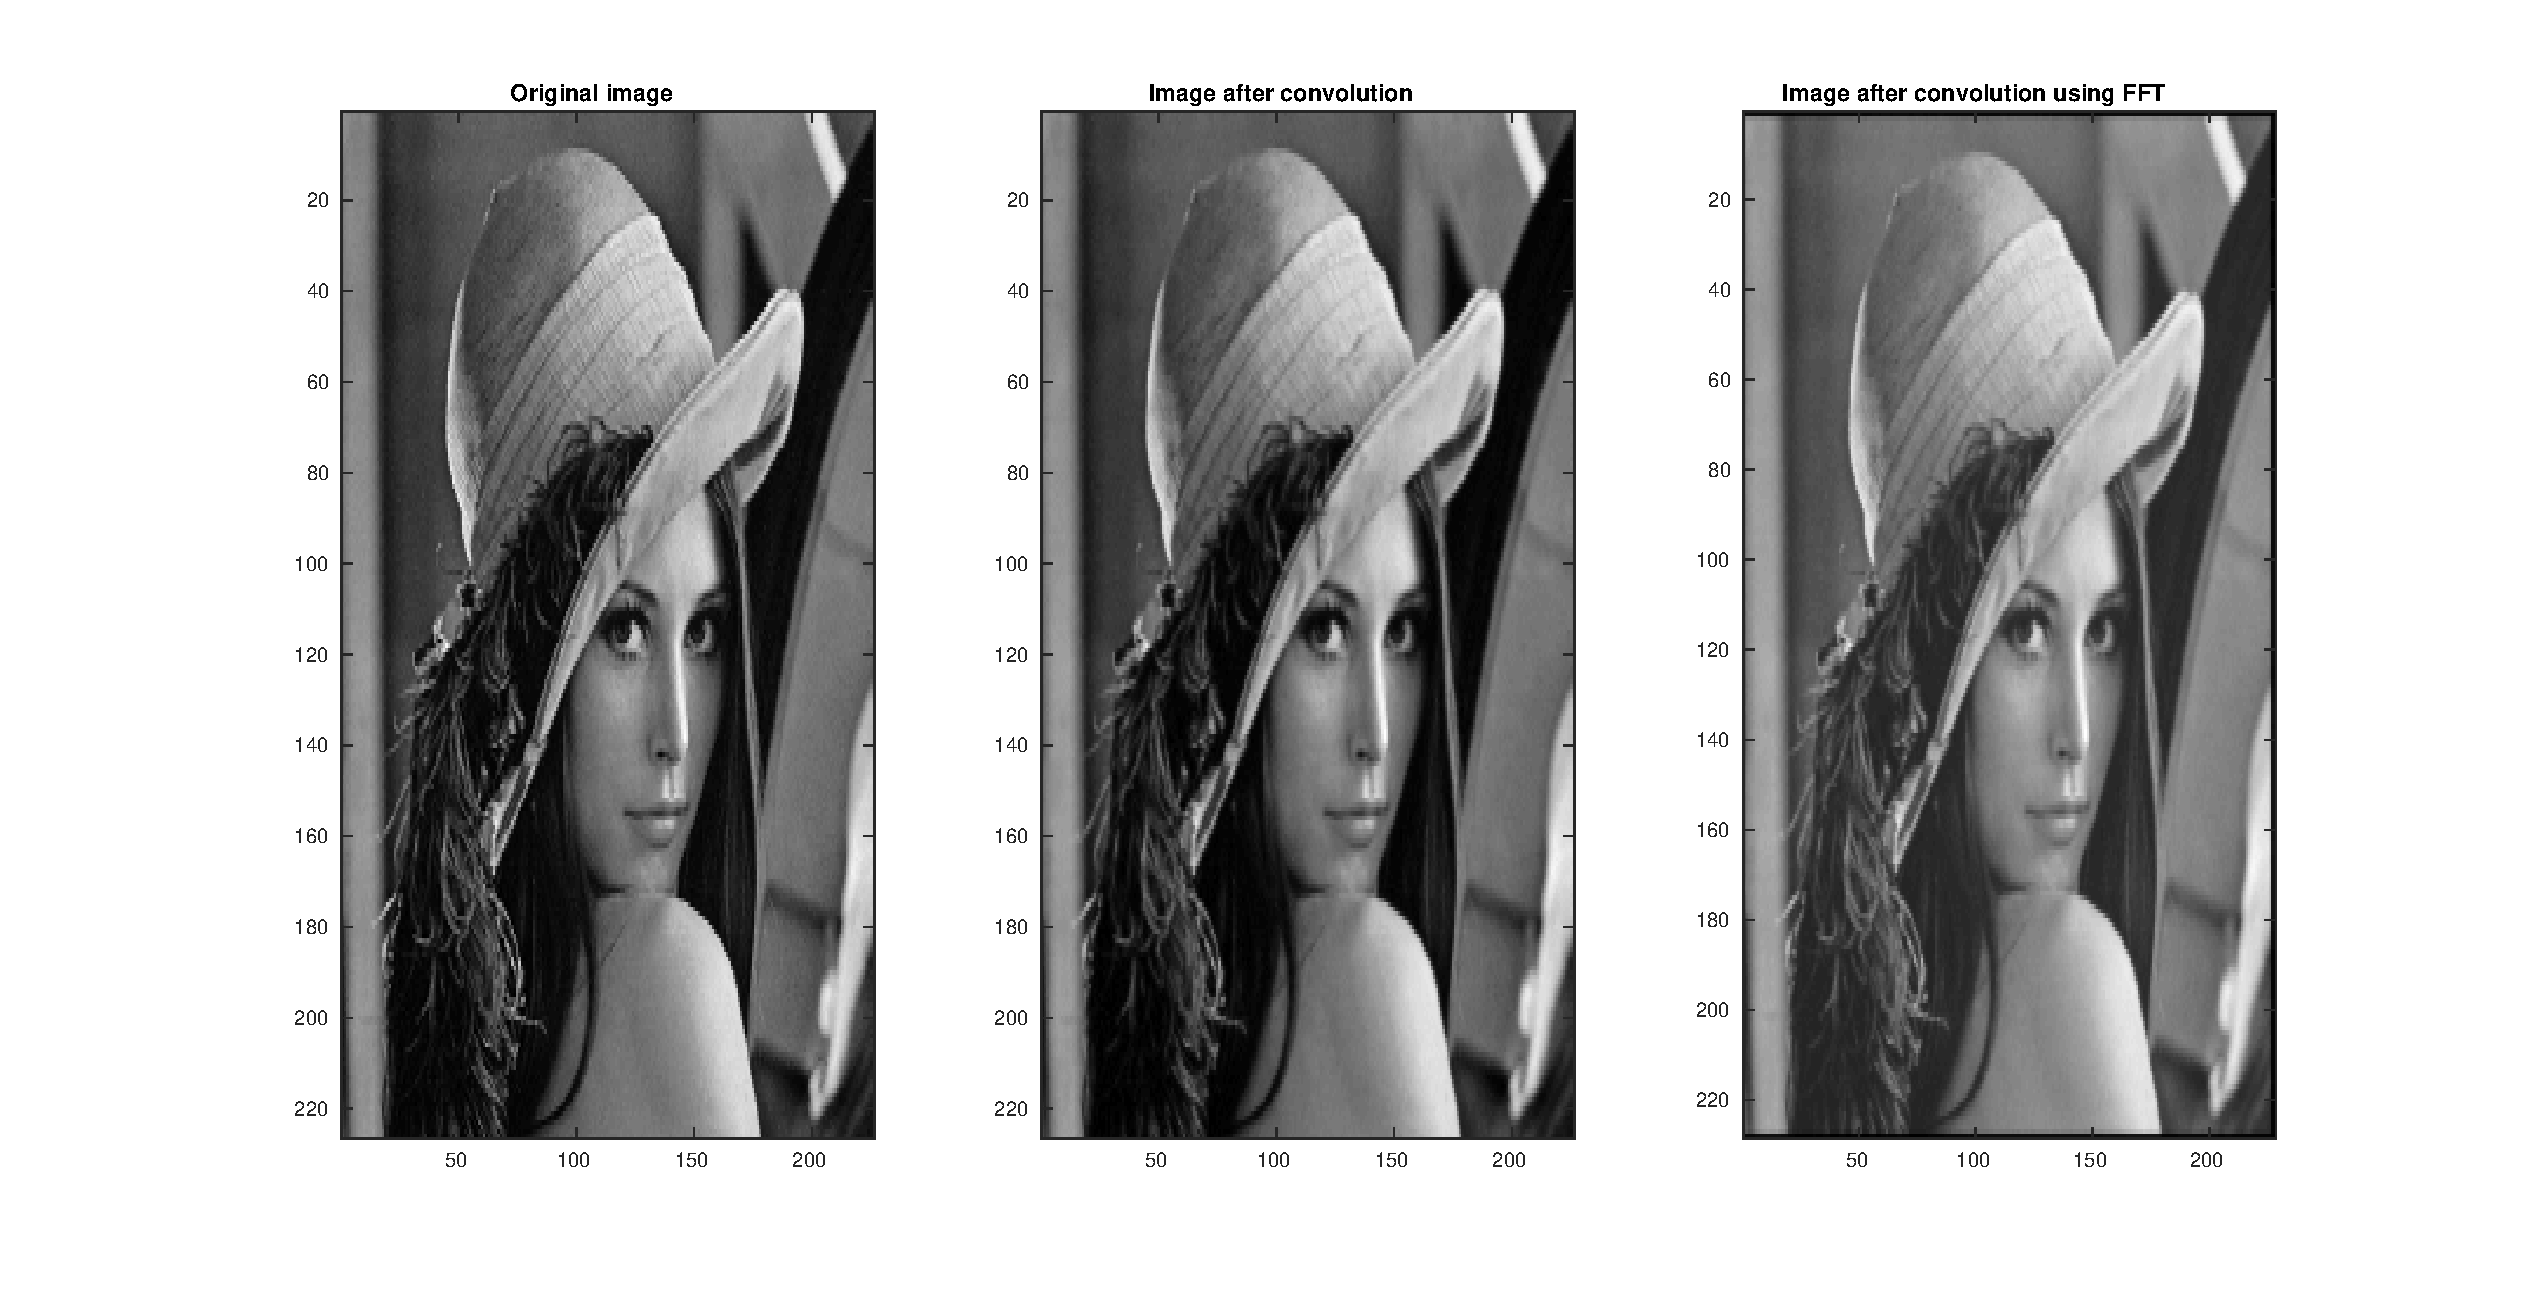
\includegraphics[width=\textwidth]{fig2_1.eps}
  \caption{Figure showing the results from using convolution using nested for loops and fast fourier transform.}
  \label{fig2_2a}
\end{figure}
Both are using a gaussian filter using a window size of $3$. Even though it might be a little hard to tell, the nested for loop result in the middle a little blurred as expected, but using FFT brightens the image as well. \\
Another result we get from running \texttt{q2\_2b} is shown in Figure \ref{fig2_2b}. It shows the computation time between the two methods depending on the window size of the kernel. For the window size of $n*n$, we use $n=\{3,5,..,15\}$.
\begin{figure}[H]
  \centering
  \captionsetup{justification=centering}
  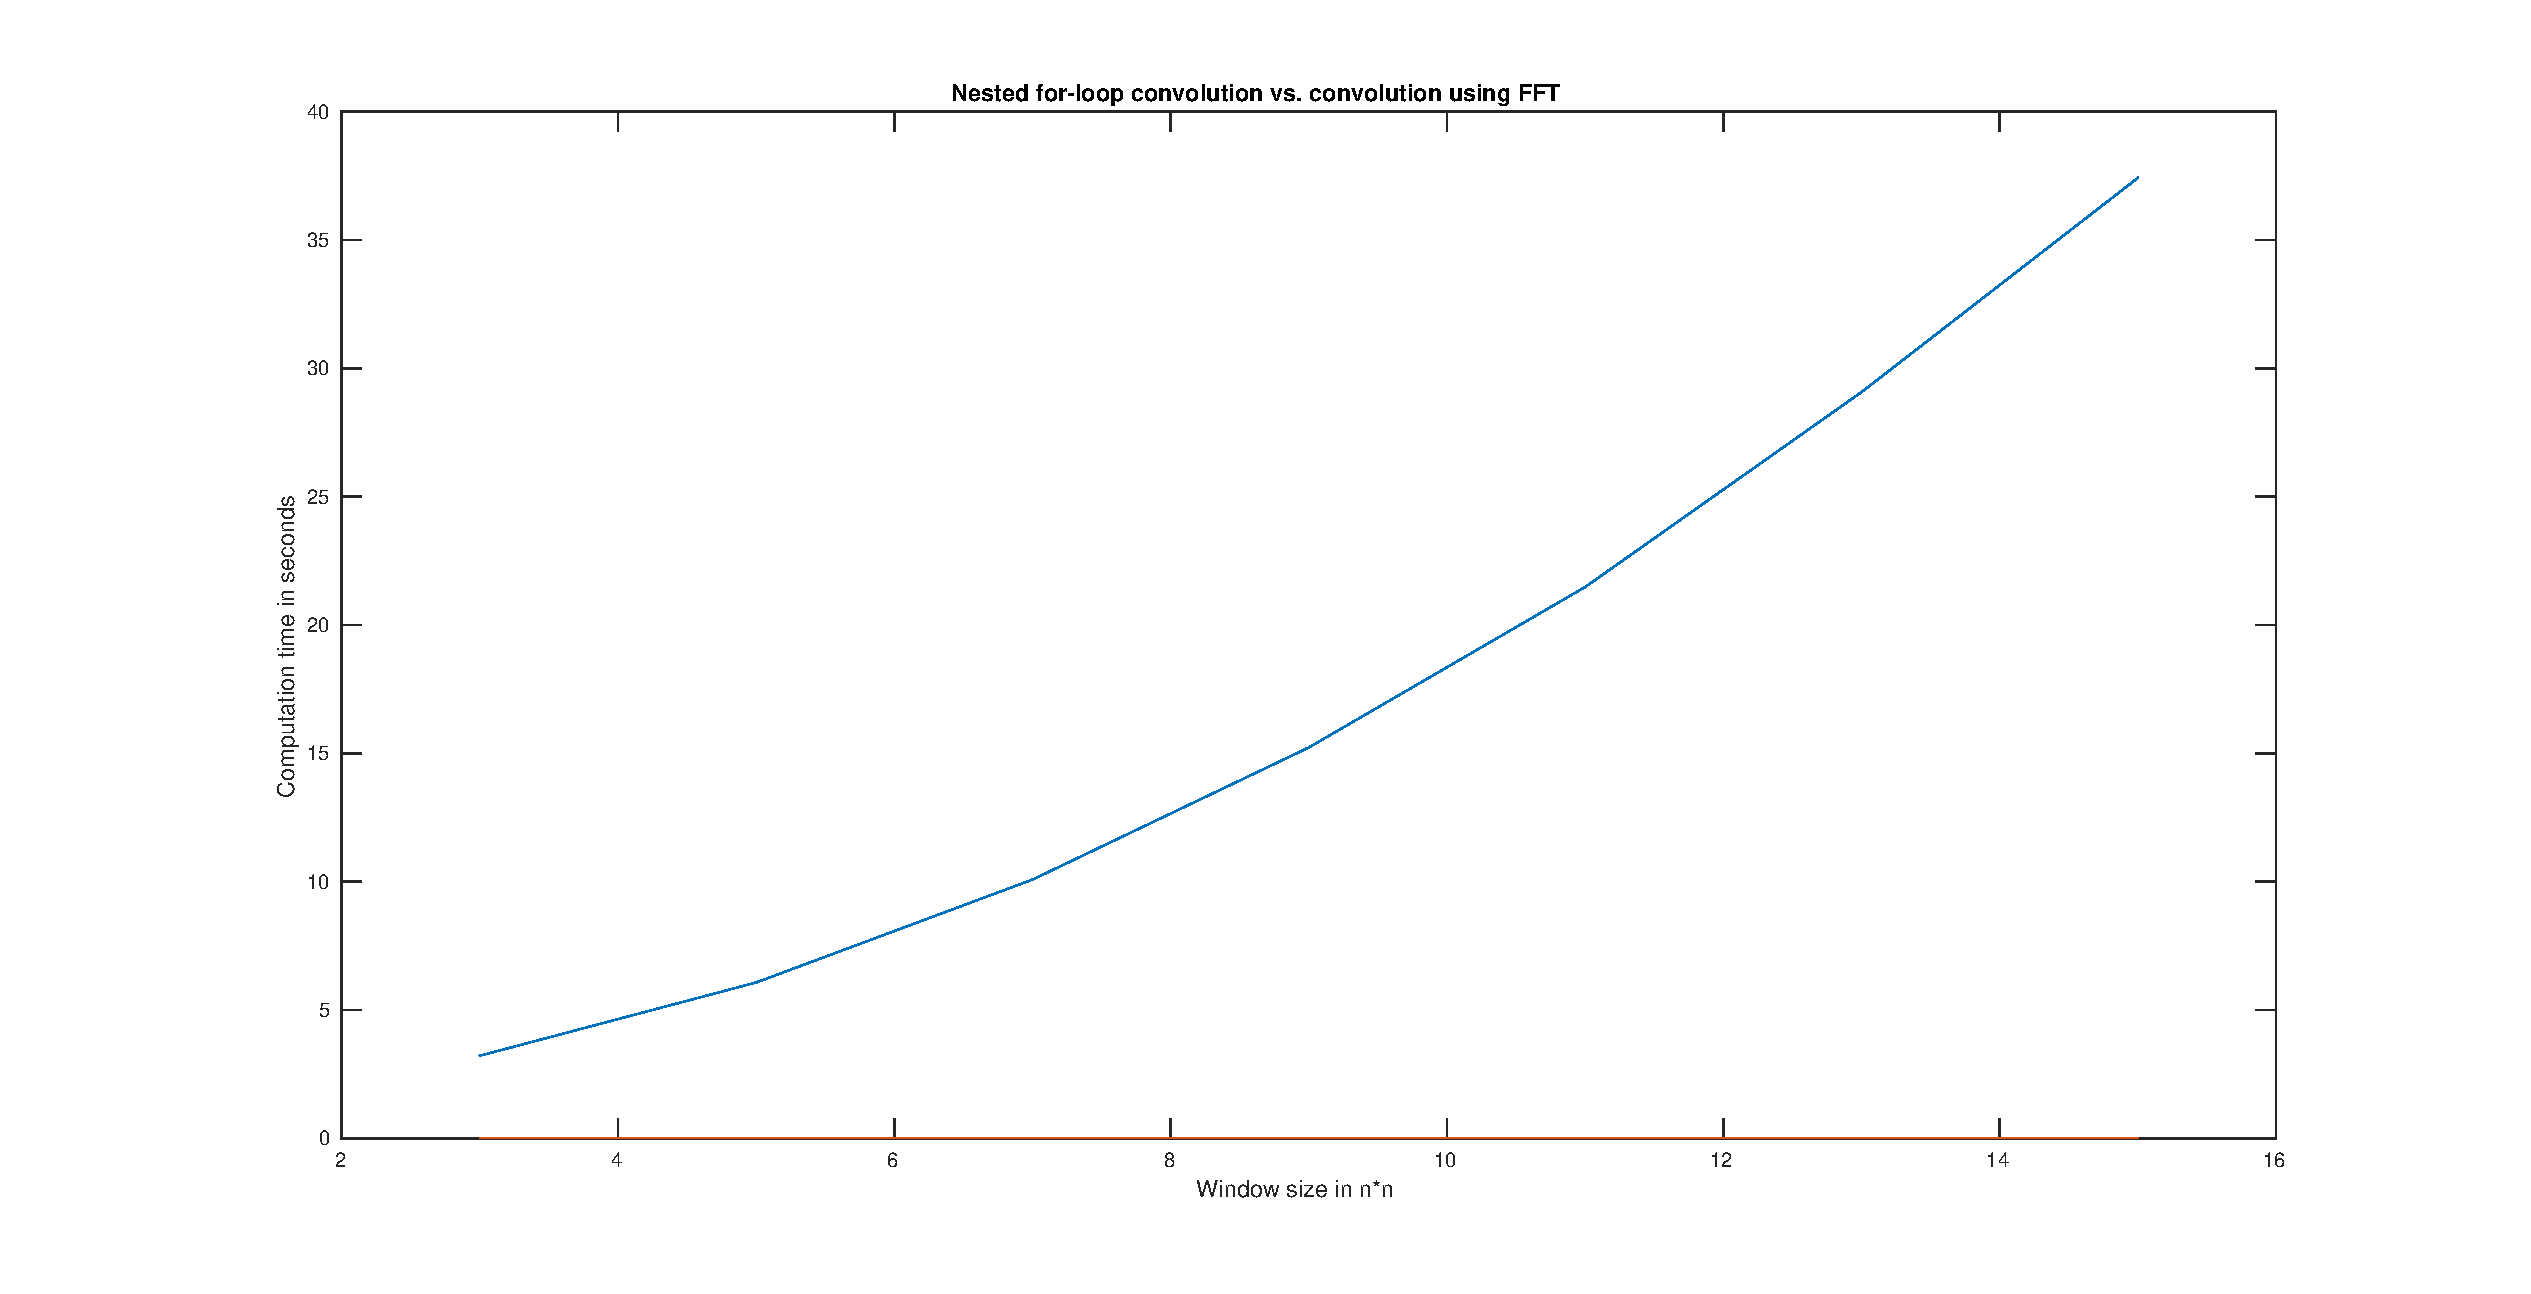
\includegraphics[width=\textwidth]{fig2_2.eps}
  \caption{Figure showing the difference in computation time for the two implemented convolution methods for different window sizes of the kernel. The blue line is the nested for loop method and the red line is the FFT method.}
  \label{fig2_2b}
\end{figure}
The blue line is the nested for loop method and the red line is the FFT method. We can see that FFT is a lot faster as it is always non existant in the plot. No matter what the window size is, it has a computation time under $1$ second. The nested for loop method is steadily increasing in computation time for increasing window size. \\
The last result in Figure \ref{fig2_2c} shows the difference in computation time for different image sizes. The image \texttt{lena.tiff} has been used with scales from $0.1$ to $1$ (where $1$ is the normal size of the image).
\begin{figure}[H]
  \centering
  \captionsetup{justification=centering}
  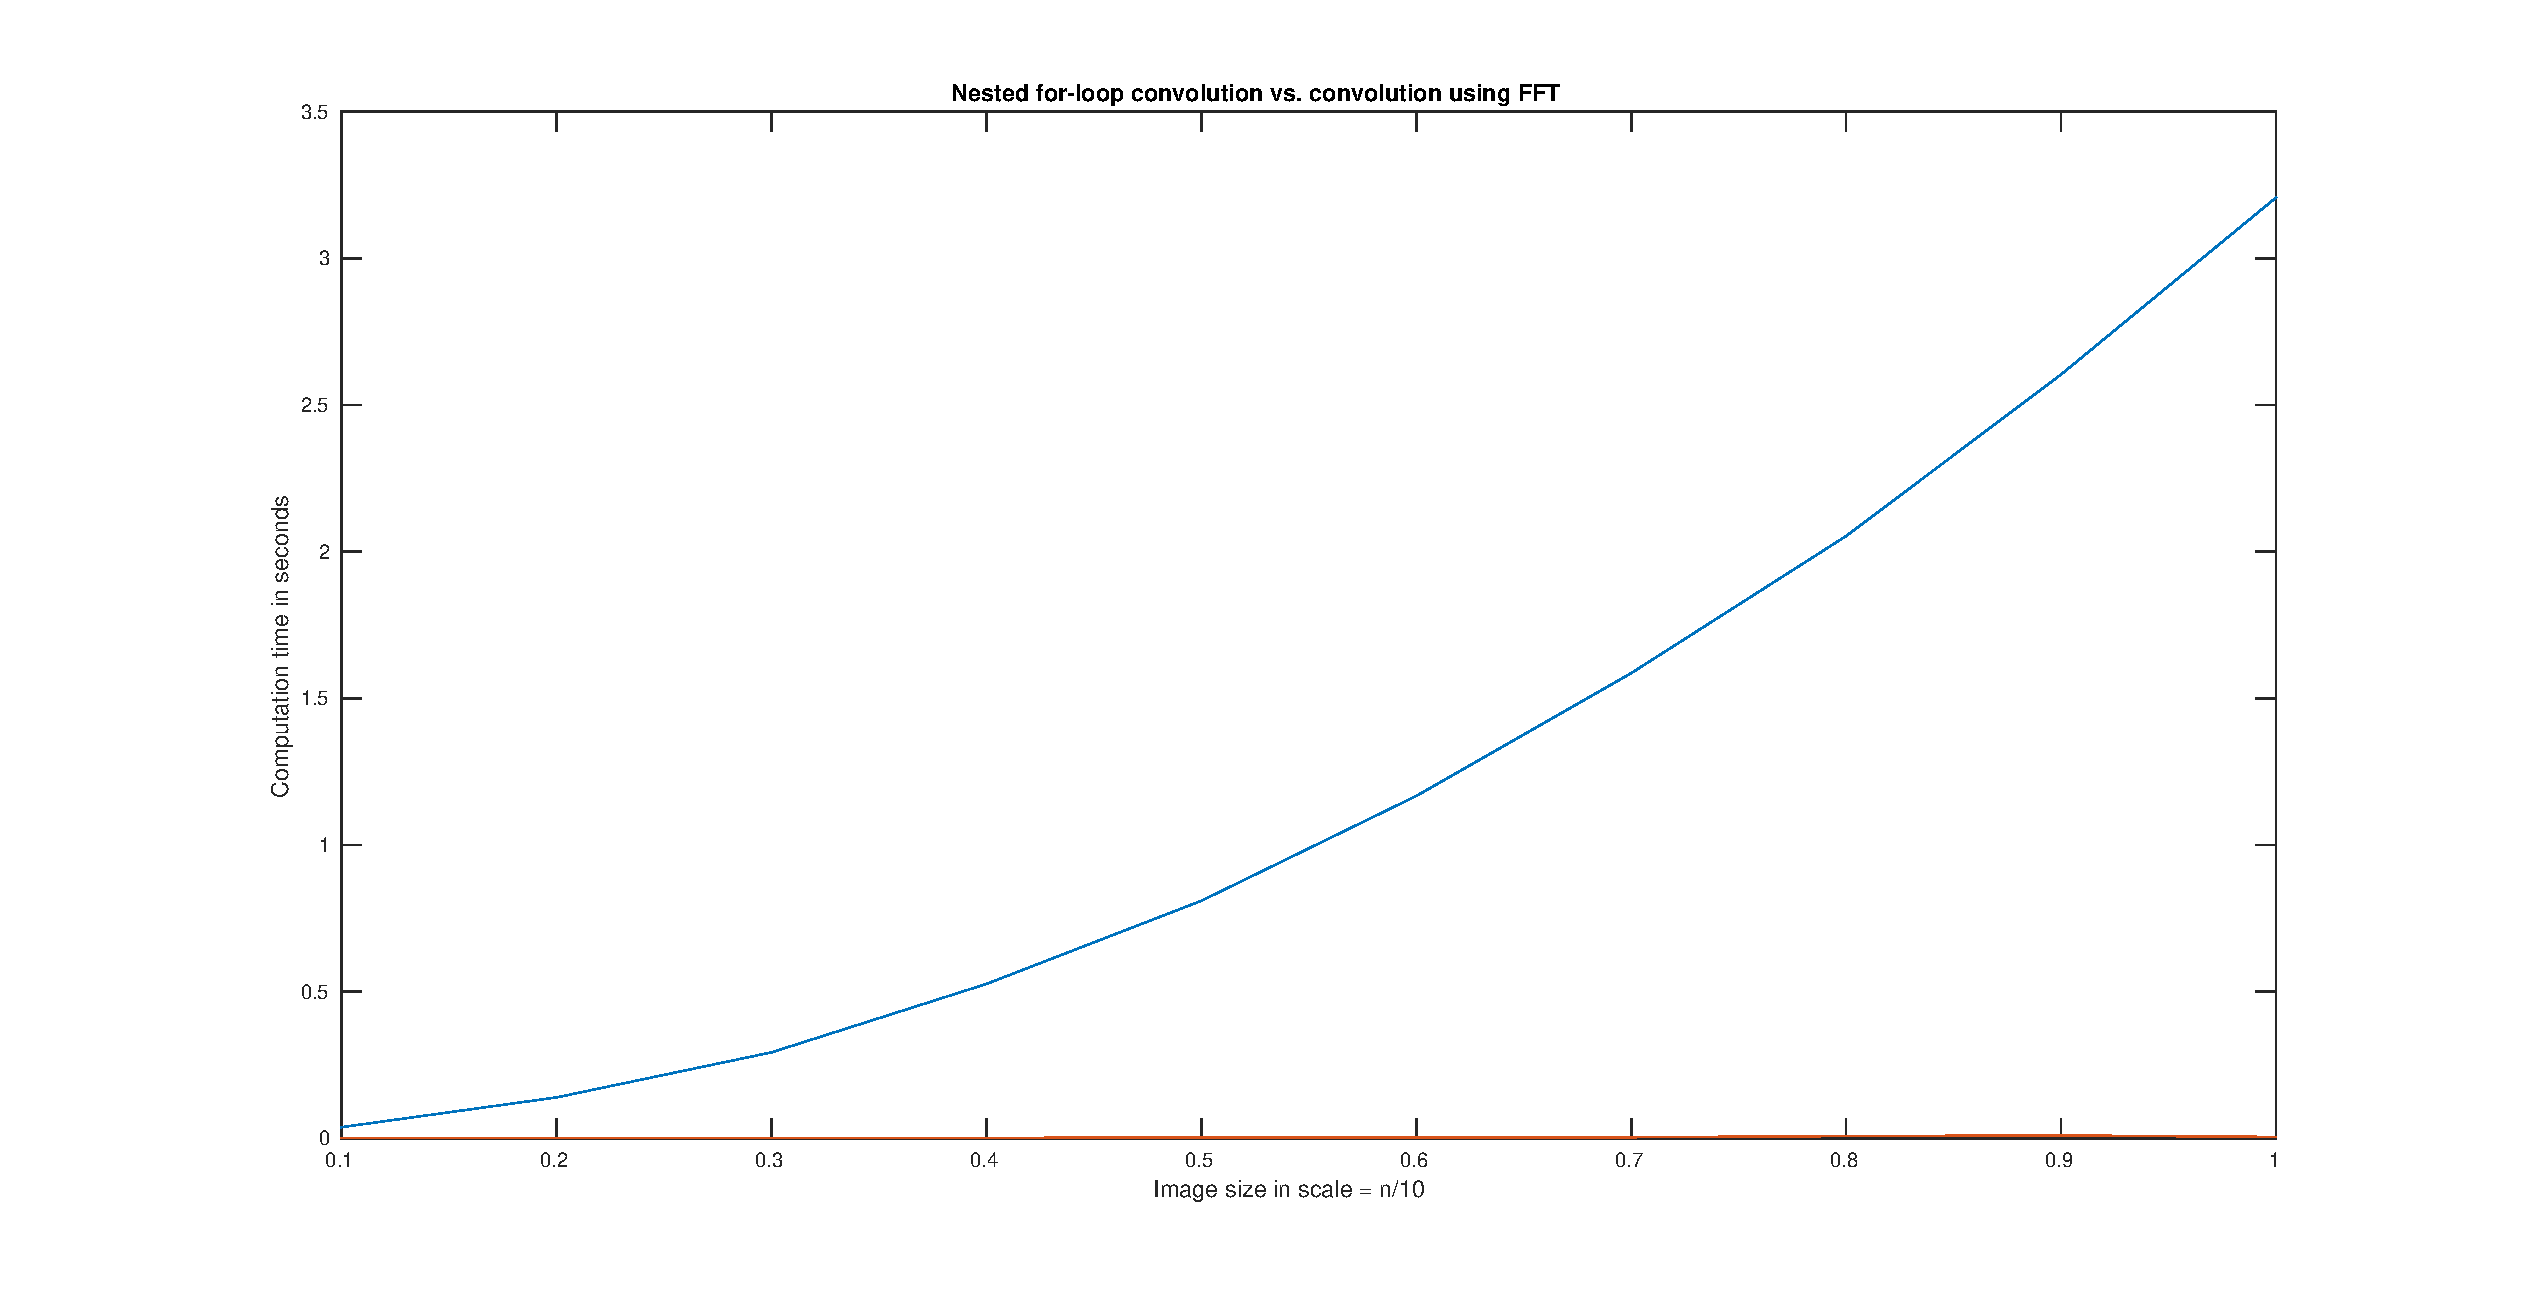
\includegraphics[width=\textwidth]{fig2_3.eps}
  \caption{Figure showing the difference in computation time for the two implemented convolution methods for different image sizes. The blue line is the nested for loop method and the red line is the FFT method.}
  \label{fig2_2b}
\end{figure}
Again the blue line is the nested for loop method and the red line is the FFT method. Once again the FFT method is way faster, while the nested for loop method is increasingsly slow. So despite brightening the image a bit, it is way faster to perform FFT compared to the nested for loop method.

\subsection{(c)}
The code for this question is seen below:
\lstinputlisting[language=Matlab]{src/q2_3.m}
The function \texttt{addFunc} adds noise depending on parameters $a$, $v$ and $w$. Running the code will generate $4$ images that can be found in Figure \ref{fig2_3} with parameters $a=50$, $v,w=0.25$.
\begin{figure}[H]
  \centering
  \captionsetup{justification=centering}
  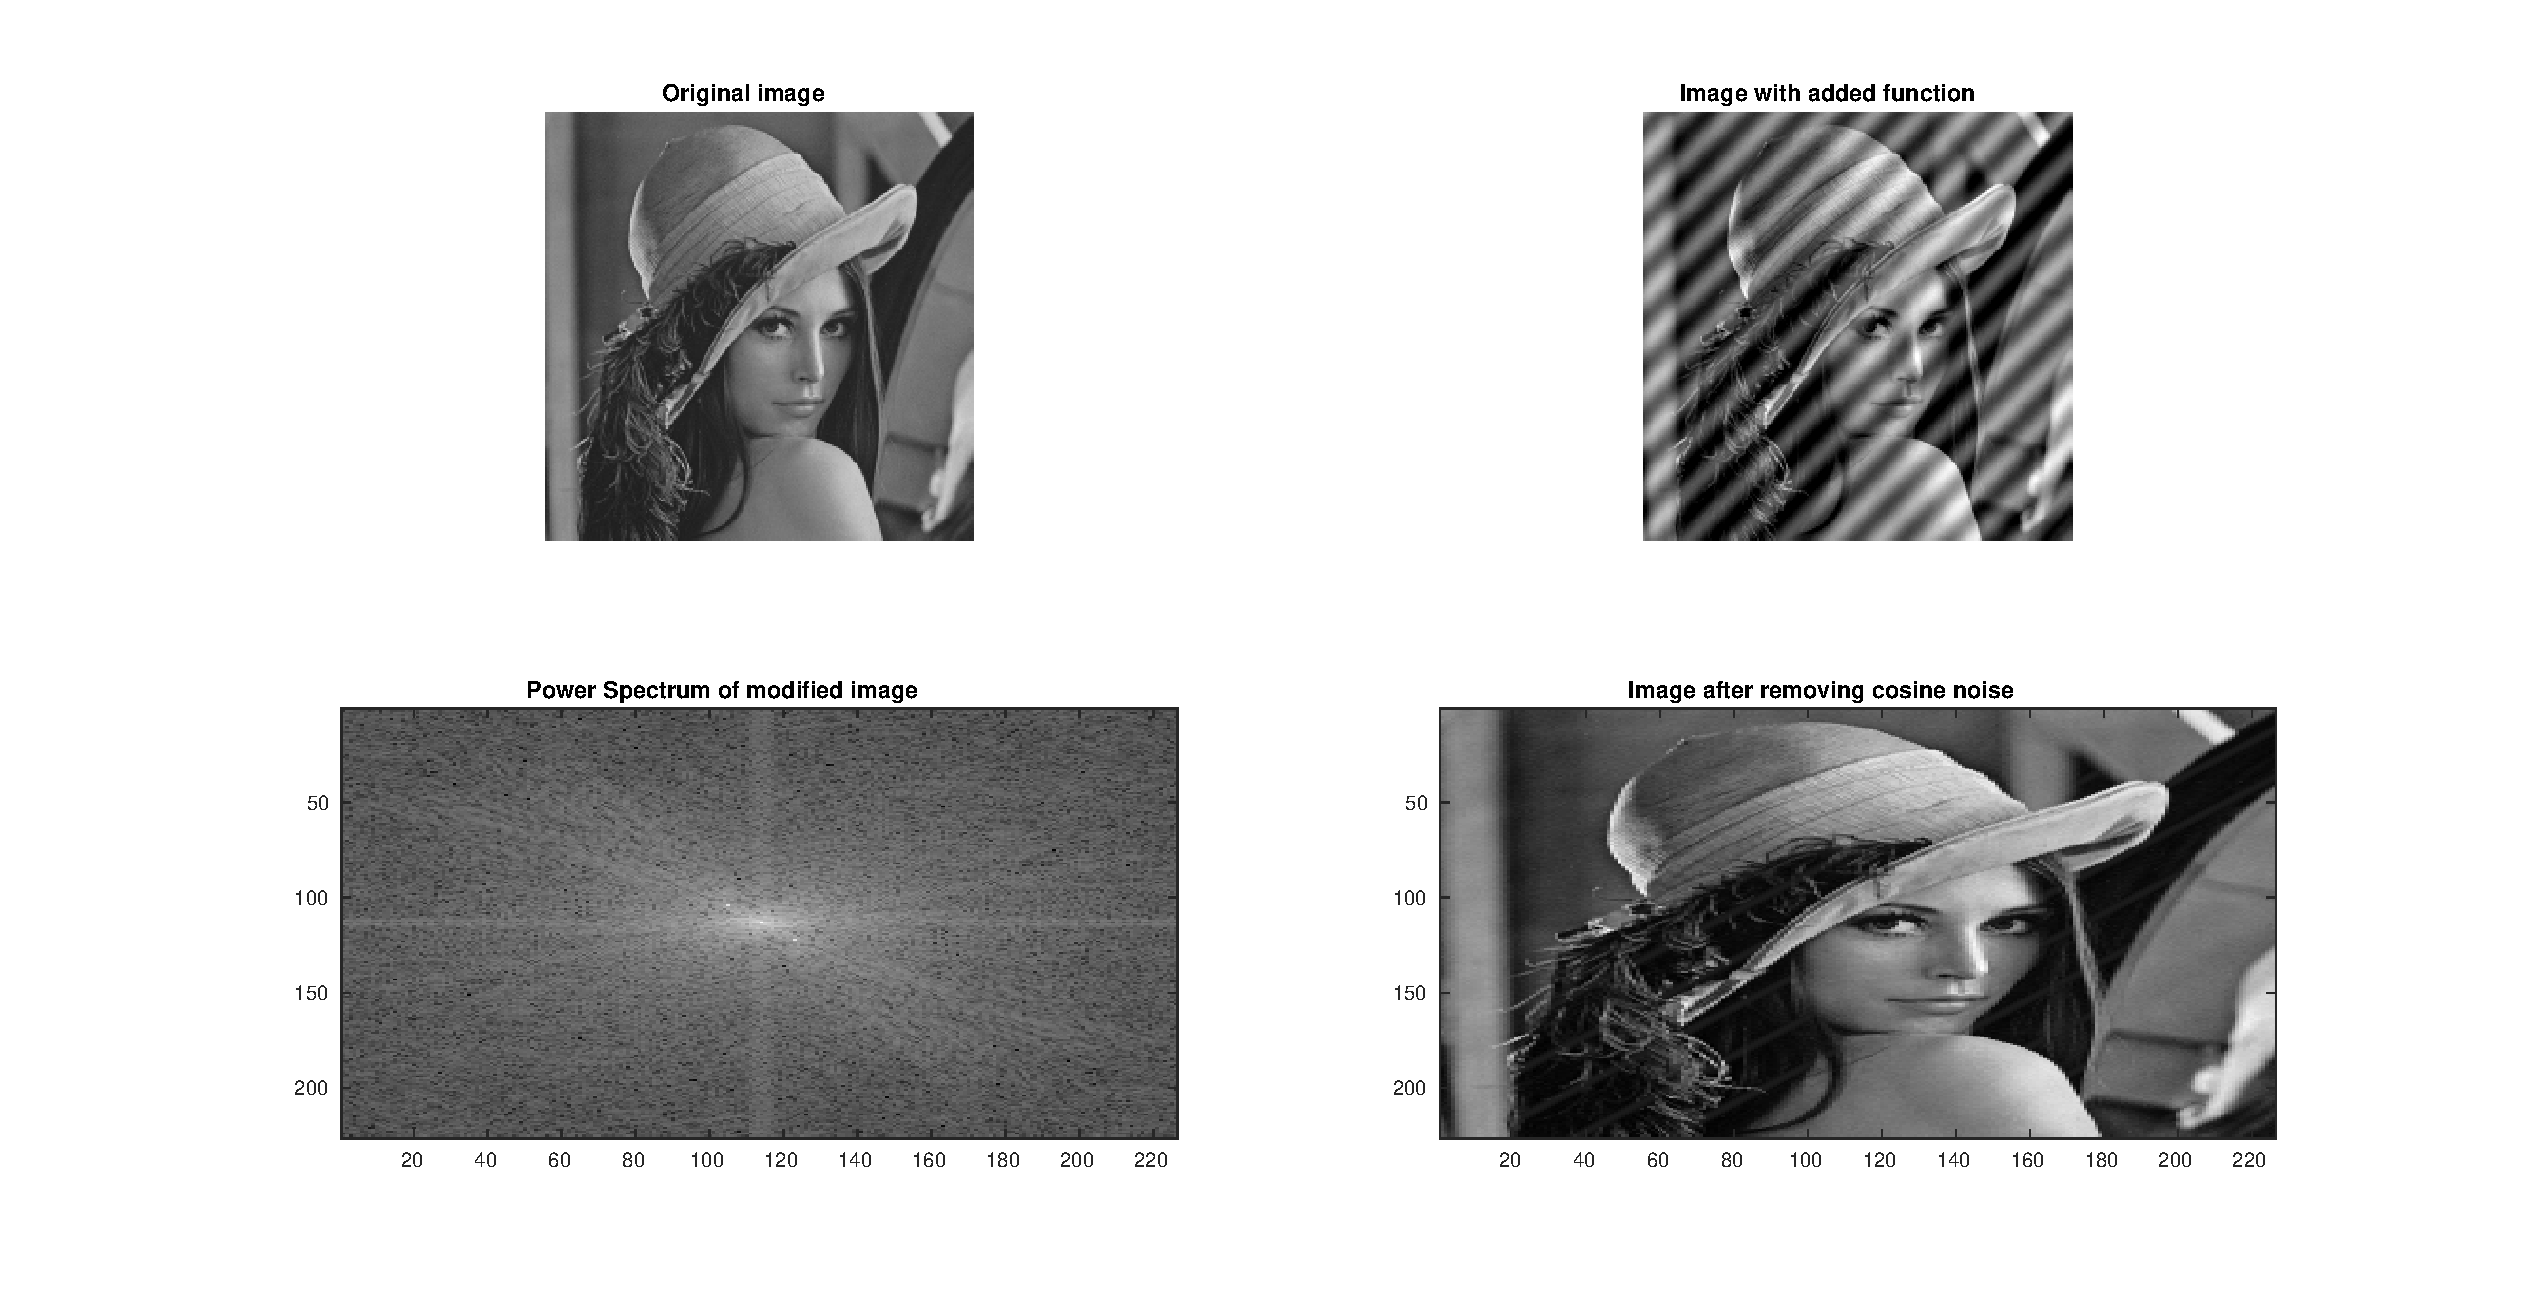
\includegraphics[width=\textwidth]{fig2_3b.eps}
  \caption{Figure showing the image \texttt{lena.tiff} along with the image with added cosinus noise. The two lower images is the power spectrum of the image with cosine noise and the image after an attempt to remove the noise from the image has been made.}
  \label{fig2_3}
\end{figure}
The upper left image is the orginal one. The upper right shows the image with added cosine noise. In the lower left, we have a power spectrum of the image with cosine noise. Again the two lines that make a plus are explained by the shifting of the image. But we can also see two very bright spots near the middle, which is the signal of the cosine noise (one for negative values and one for positive values). To remove this noise, a very simple solution exists by changing pixel value for this signal. Doing this results in the image in the lower right. Even though it might seem very clean, there are actually still some grey lines going from the lower left corner to the upper right corner, which means the signal is still somewhat present in the image.

\subsection{(d)}
The function \texttt{scale} is implemented as below:
\lstinputlisting[language=Matlab]{src/q2_4.m}
The first function \texttt{q2\_4} is responsible for plotting, while the \texttt{scale} function is implemented such that it take an argument (sigma), and performs gaussian filtering on the image \texttt{lena.tiff}. Since using a fixed window size for the kernel would result in almost identical images, the window size is set to the value of sigma as well. This resulted in Figure \ref{fig4}.
\begin{figure}[H]
  \centering
  \captionsetup{justification=centering}
  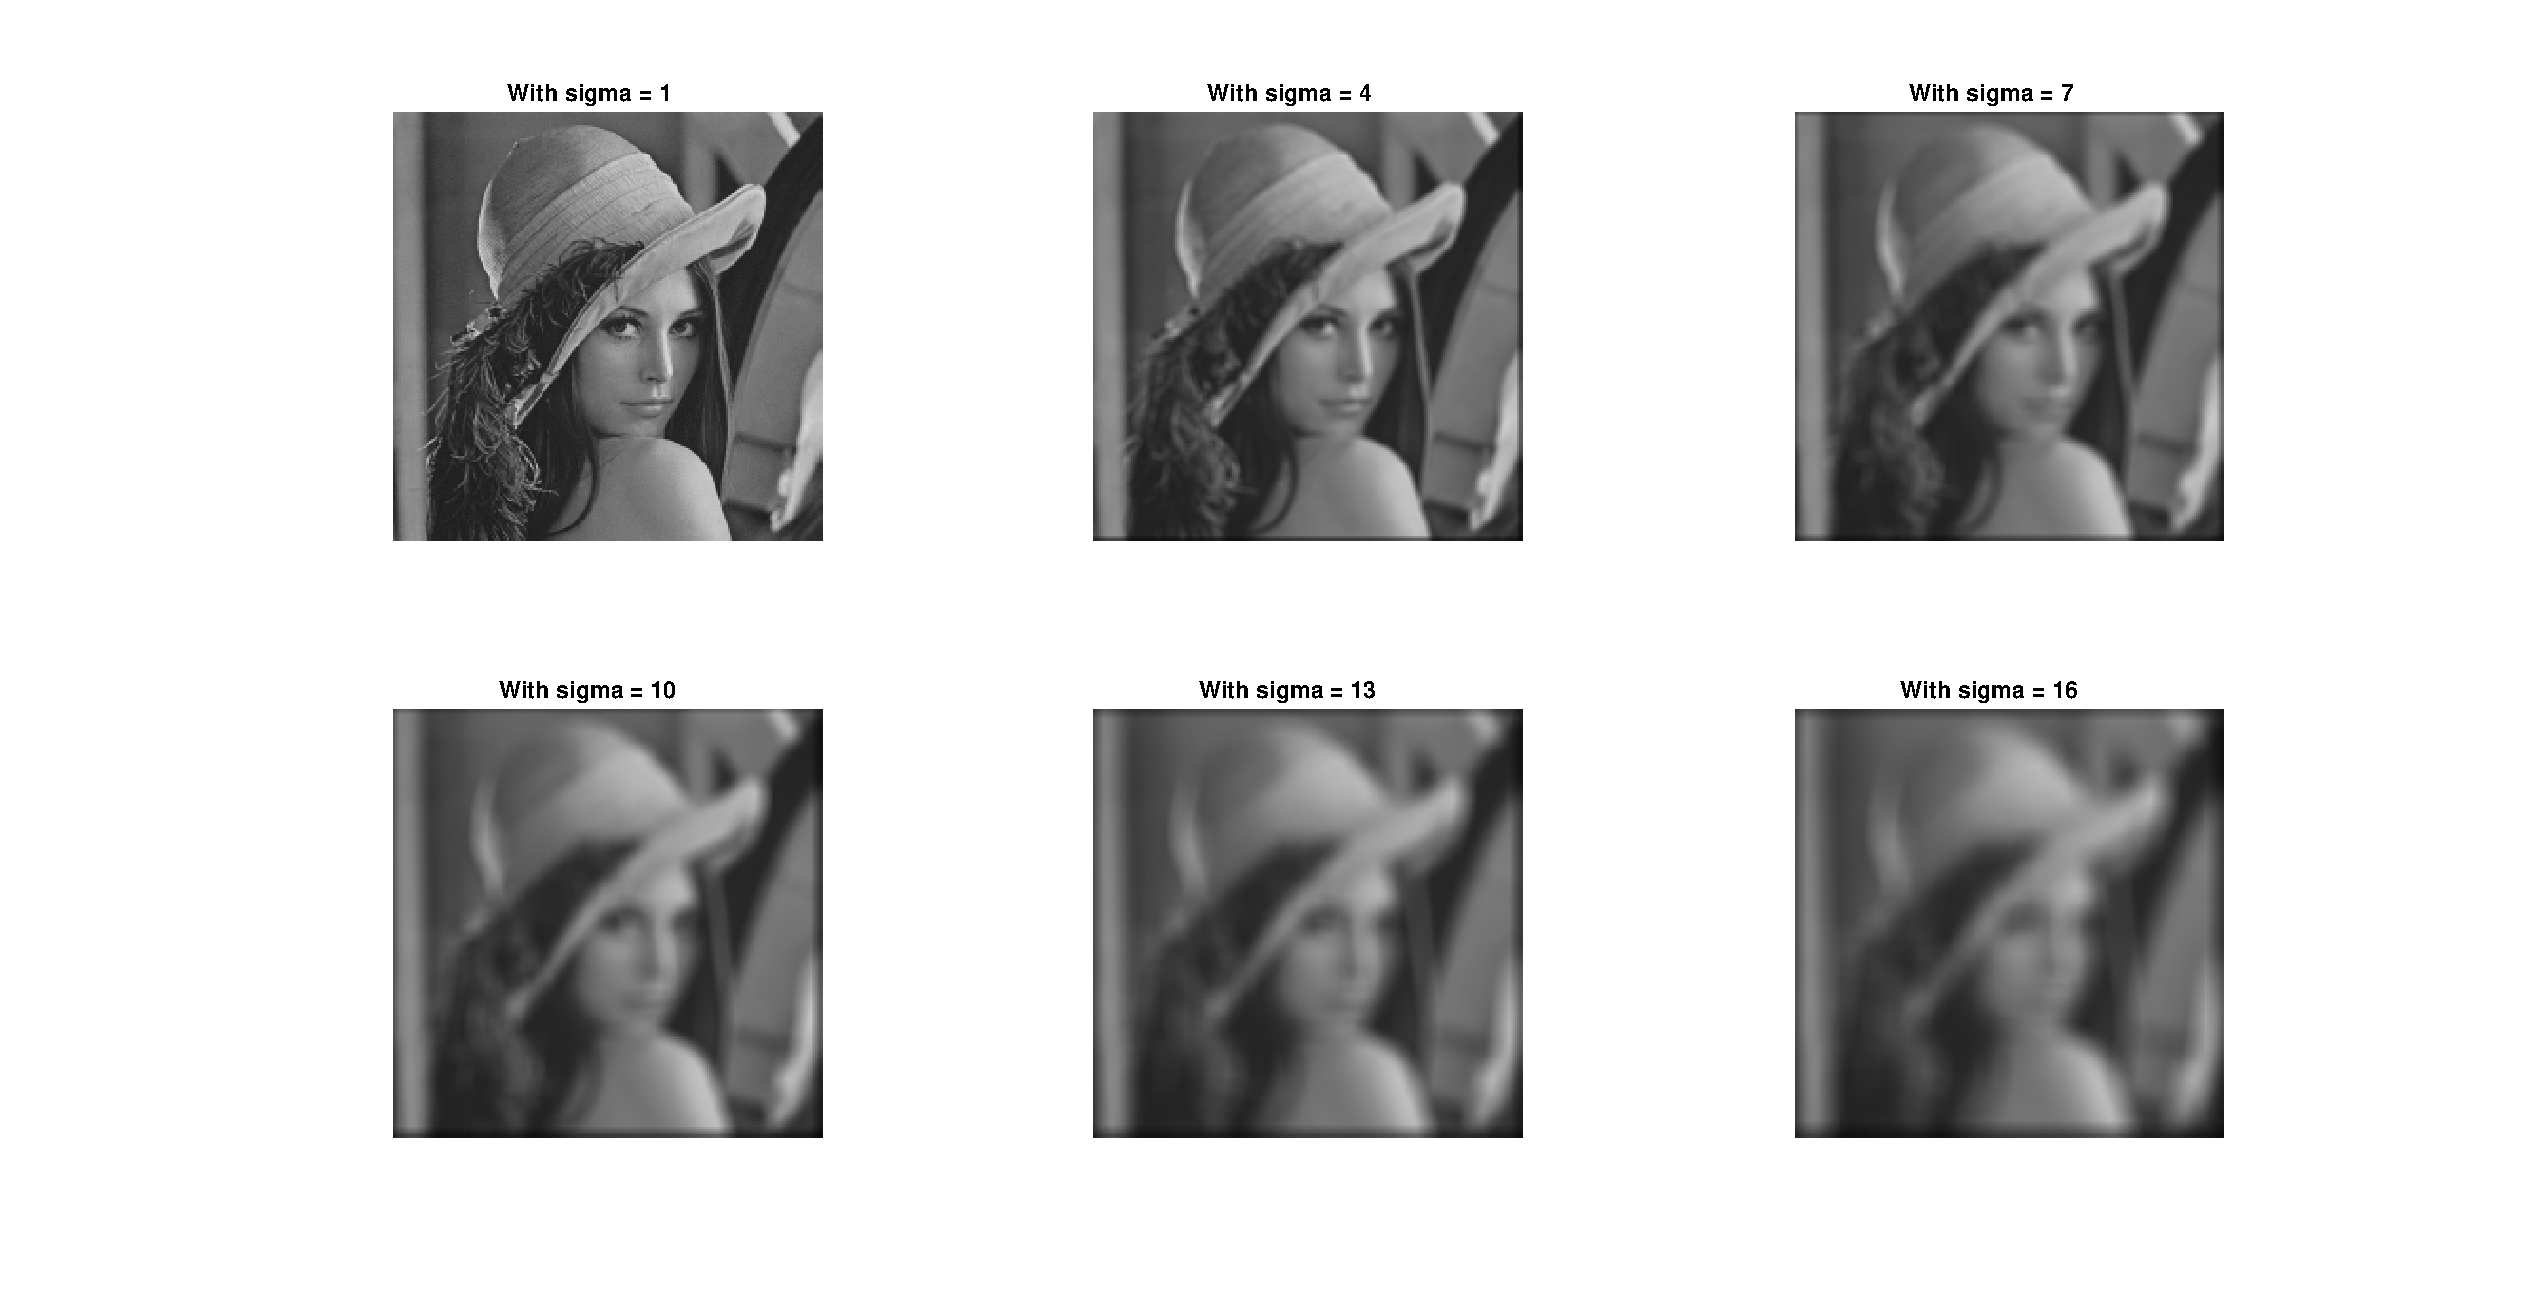
\includegraphics[width=\textwidth]{fig4.eps}
  \caption{Figure showing the difference of sigma and window size when performing gaussian filtering on the image \texttt{lena.tiff}.}
  \label{fig4}
\end{figure}
As expected, the image becomes more blurry as neighbouring pixels are weighted higher, and as such, they have a larger impact on the pixel we are looking at.

\subsection{(e)}
We want to show that the spatial derivatives of a function $f(x)$ can be written as a multiplication of a kernel in the fourier domain. We have the fourier transform of $f$ is given by:
\begin{align*}
  F(k_x)=\frac{1}{2\pi}\int f(x)e^{-ik_xx}dx
\end{align*}
We now have that
\begin{align*}
  F(f')(k_x)&= \frac{1}{2\pi}\int f'(x)e^{-ik_xx}dx \\
        &= \frac{1}{2\pi}\int ik_xf(x)e^{-ik_xx}dx
\end{align*}
Since the derivative of the exponential simply taking the constants in the power down. Since these are constants we can write:
\begin{align*}
  F(f')(k_x) &= \frac{1}{2\pi}\int ik_xf(x)e^{-ik_xx}dx \\
         &= ik_x\cdot \frac{1}{2\pi}\int f(x)e^{-ik_xx}dx \\
         &= ik_x\cdot F(f)(k_x)
\end{align*}
which is what we wanted to show. This relation can be used when we want to find more than one order of derivatives, since it is a lot easier and faster to find derivates this way than to compute them in a traditional way every time.

\subsection{(f)}
To generalize on the derivation we made in (2.5), we can see that the derivative of order $n$ can be found by just multiplying with the constants $n$ times, i.e. we can find the derivative of order $2$ by $ik_x^2\cdot F(f)(k_x)$ in the derivation made above. When we want to take the derivative of an image, we are not looking at a function $f(x)$, but a function $f(x,y)$. The derivation we made above still applies, which means what we want to calculate is actually
\begin{align*}
  ik_x\cdot ik_y F(f(k_x, k_y))
\end{align*}
For order $1$, and
\begin{align*}
  (ik_x)^n\cdot (ik_y)^m F(f(k_x, k_y))
\end{align*}
For two given order $n$ and $m$. This calculation has been implemented in Matlab as seen below:
\lstinputlisting[language=Matlab]{src/q2_6.m}
Note that $1j$ correspond to the imaginary part in Matlab. The function \texttt{deriveImg} is the function that makes the above calculation, while \texttt{q2\_6} simply make the plot with different parameters. The image \texttt{lena.tiff} has been used and the derivative of the image with varying derivative orders can be seen in Figure \ref{fig2_6}.
\begin{figure}[H]
  \centering
  \captionsetup{justification=centering}
  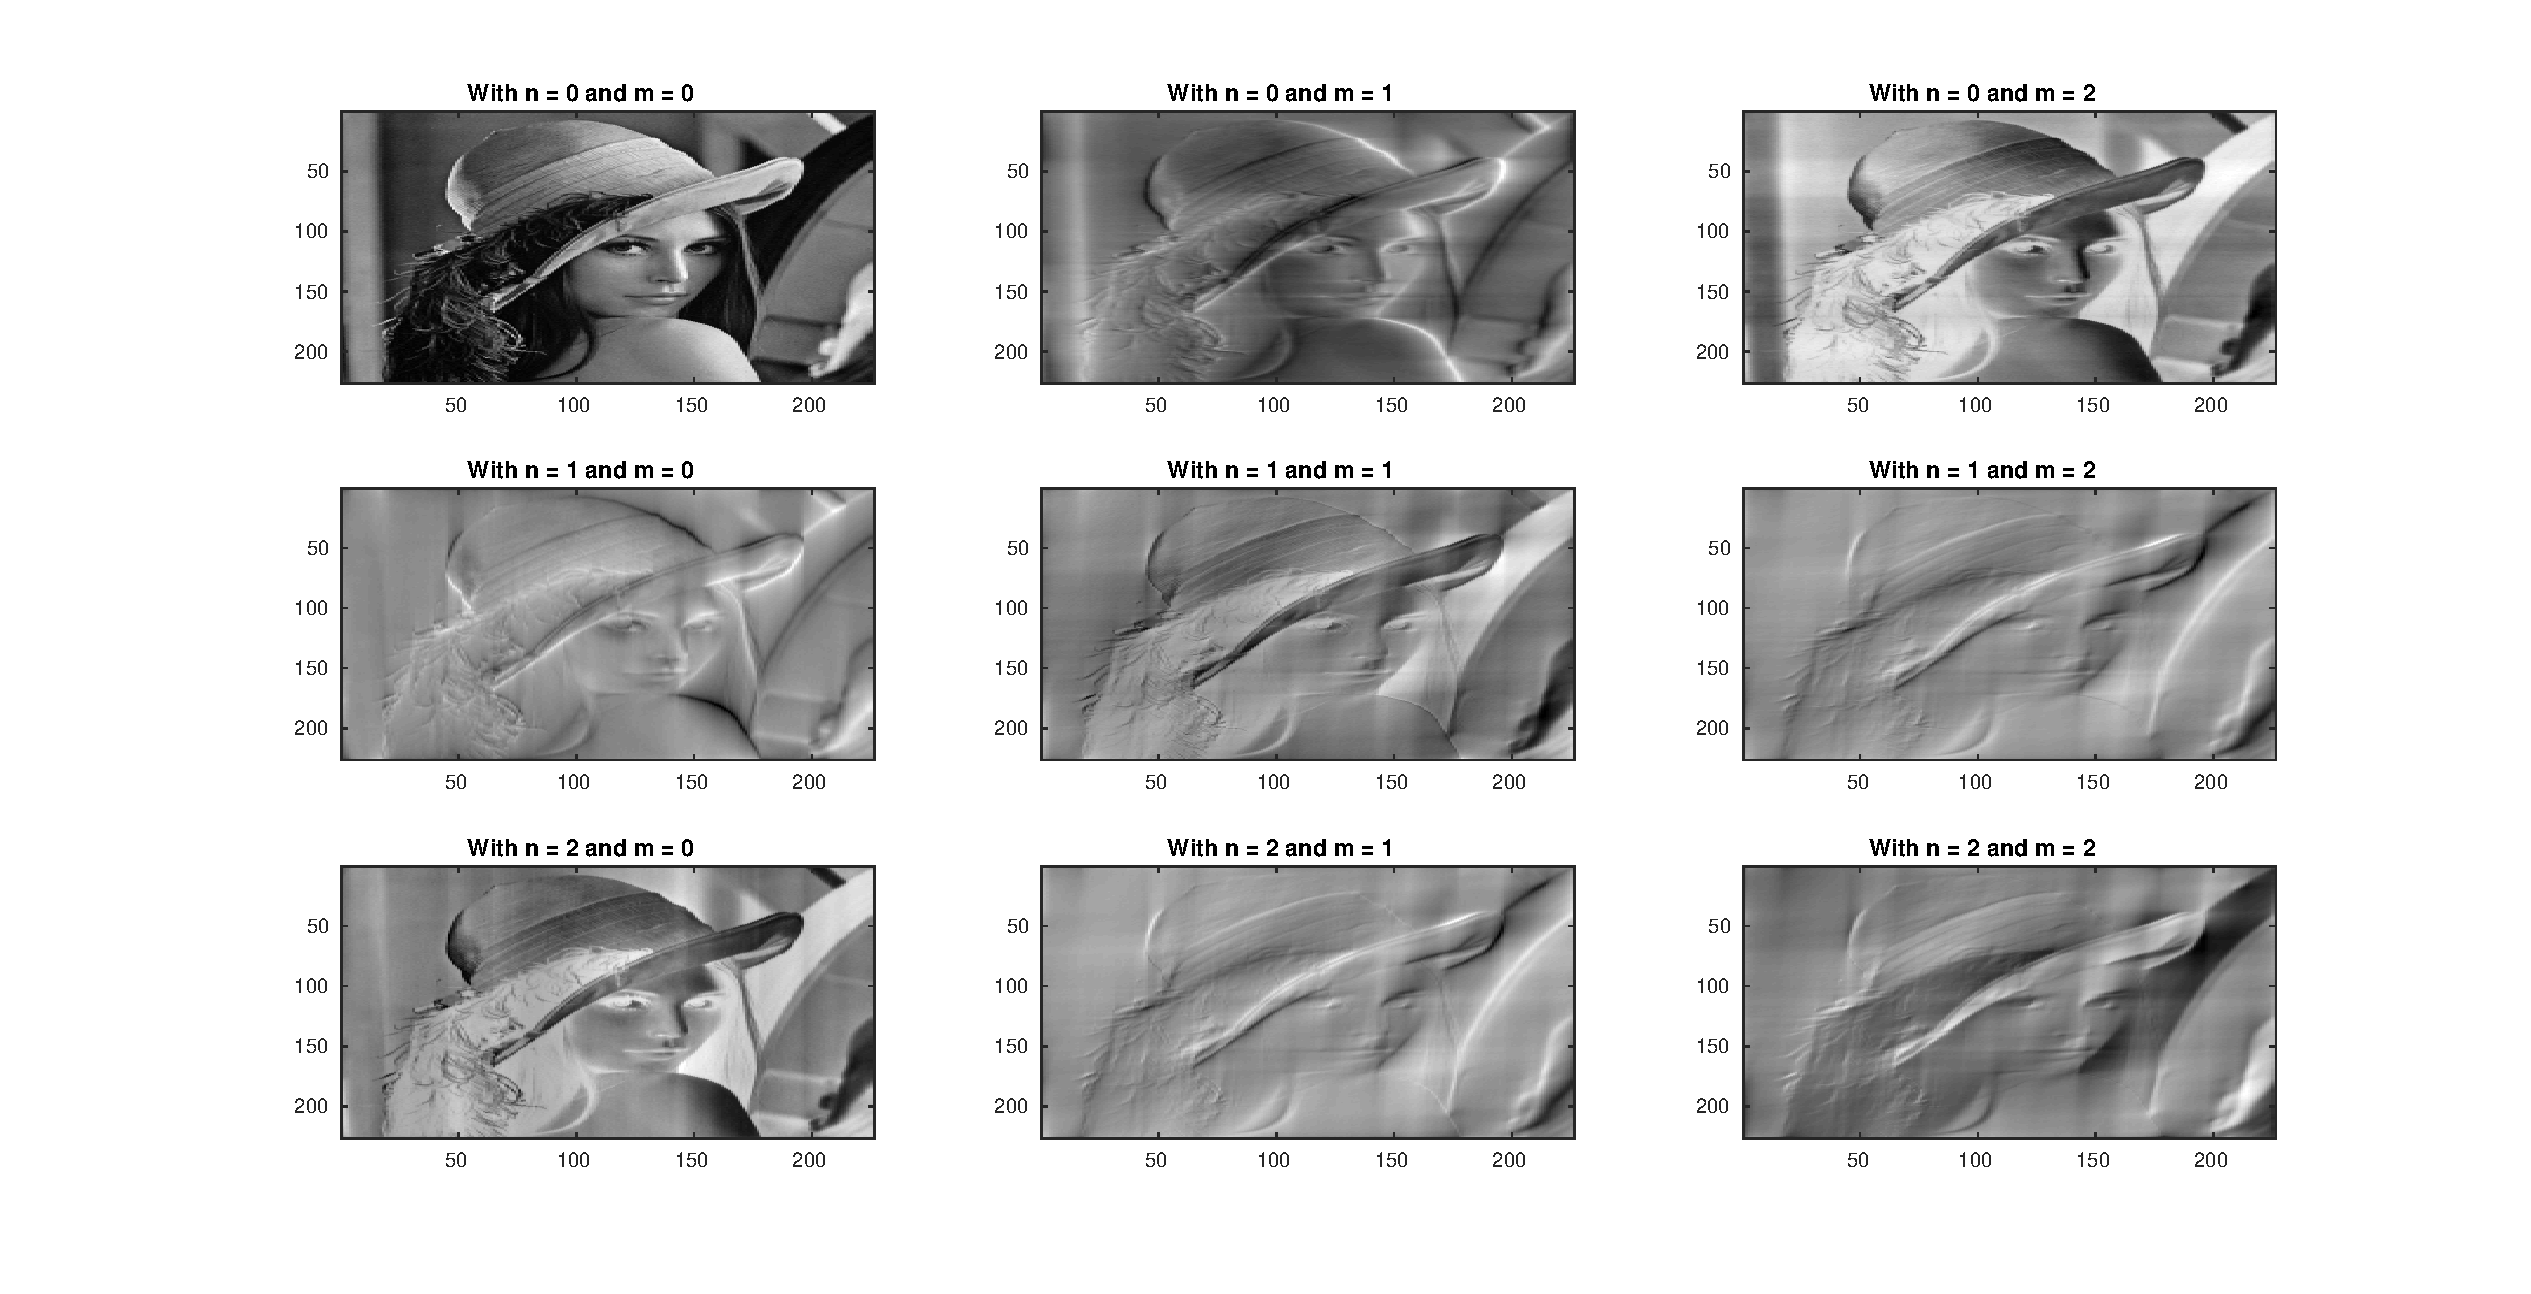
\includegraphics[width=\textwidth]{fig2_6.eps}
  \caption{Figure showing the derivative of the image \texttt{lena.tiff} with different derivative orders.}
  \label{fig2_6}
\end{figure}
We can see that a difference in the order of the two derivatives seem to negate the image. It is hard to say anything about the rest, but the higher the order, the plainer it looks. However, it seems that it can be more similar if we increase the parameters by the last image.

\end{document}
